\subsection{Computation of mode shapes}
\label{subsec:mode_shapes}

The mode shapes of the system can be computed again by considering the system of Equations \ref{eq:linear_system}.

In particular, given that to each natural frequency $\omega_n$ corresponds a mode shape, we can compute the mode shapes by solving the linear system for each natural frequency.
However, even if the system is exactly the same, it's important to understand that our goal now is to find the values of $A$, $B$, $C$ and $D$ that satisfy the system of equations, rather that finding the natural frequencies that cancel $H$.

In the end we will have a set of mode shapes, each one corresponding to a natural frequency of the system:

\begin{equation}
    H(\omega_{n, i}) z_i = 0
\end{equation}

By imposing the first component of the solution vector $z_i$ to be $A = 1$, we can find the other components of the solution vector.

\begin{equation}
    [H(\omega_{n, i})] z_i
    \rightarrow
    \hat z_i
    =
    \begin{bmatrix}
        B \\
        C \\
        D
    \end{bmatrix}
    =
    - \begin{bmatrix}
        1               & 0                & 1                \\
        -\sin(\gamma L) & +\cosh(\gamma L) & +\sinh(\gamma L) \\
        -\cos(\gamma L) & +\sinh(\gamma L) & +\cosh(\gamma L)
    \end{bmatrix}^{-1}
    \begin{bmatrix}
        0               \\
        -\cos(\gamma L) \\
        +\sin(\gamma L)
    \end{bmatrix}
    \label{eq:linear_system_for_mode_shapes}
\end{equation}

Once all the mode shapes coefficients ($A = 1$, $B$, $C$ and $D$) are computed, we can plot them with the indication of the associated natural frequency (see Figure \ref{fig:ideal_mode_shapes}).

\begin{figure}[H]
    \begin{minipage}[b]{0.45\textwidth}
        \centering
        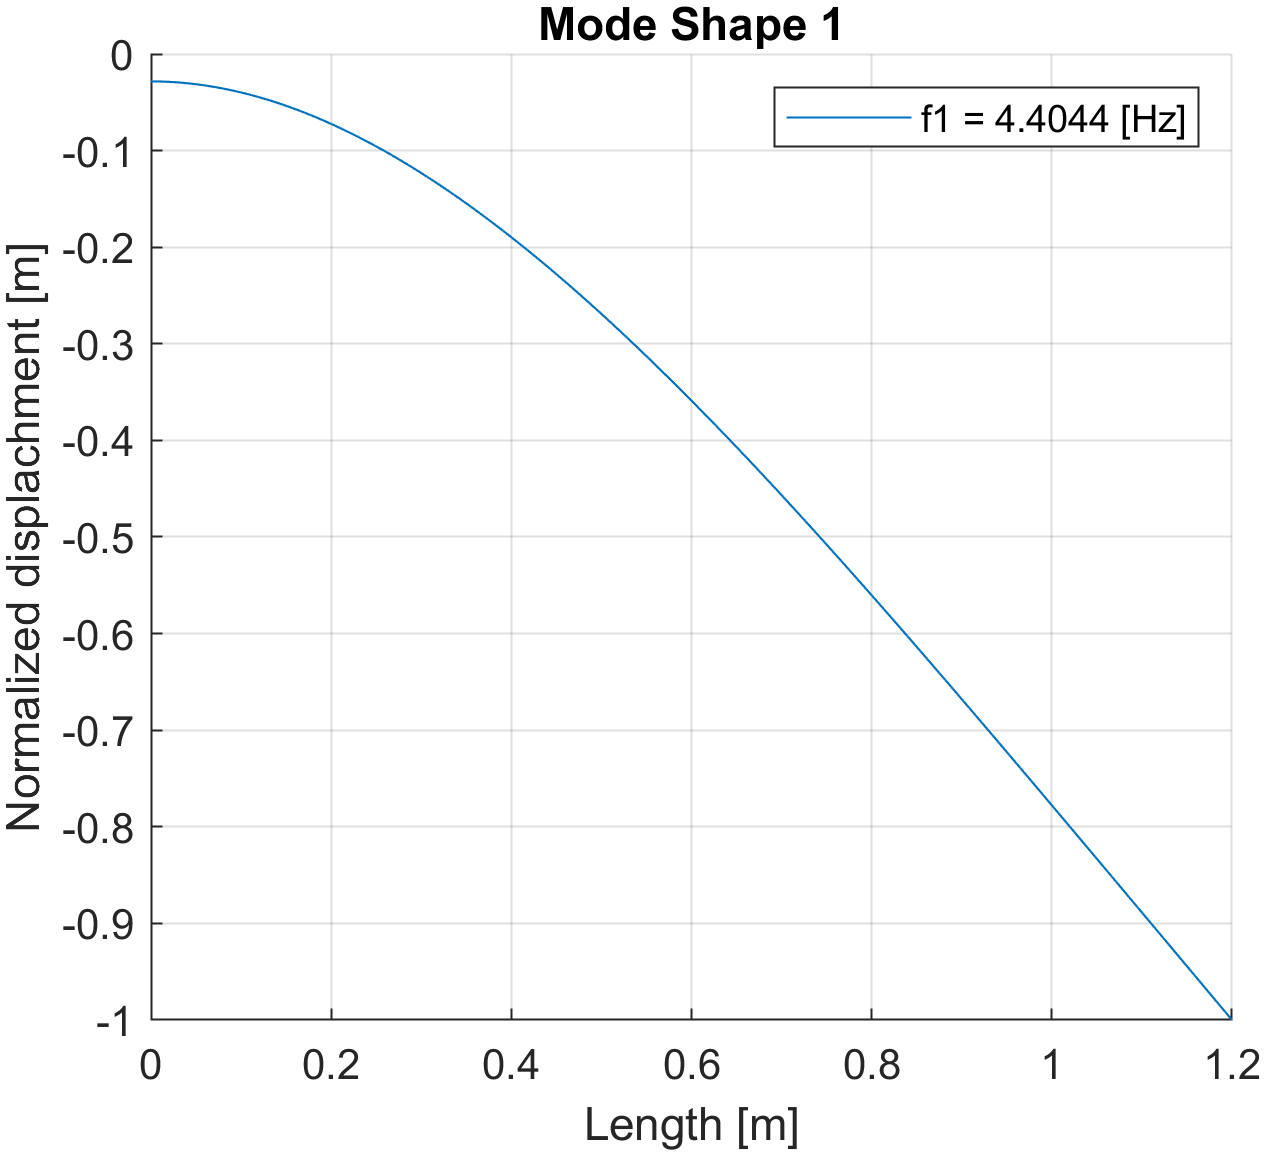
\includegraphics[width=0.9\textwidth]{img/MATLAB/Part_A/Mode_shapes/mode_shape_01.png}
    \end{minipage}
    \hfill
    \begin{minipage}[b]{0.45\textwidth}
        \centering
        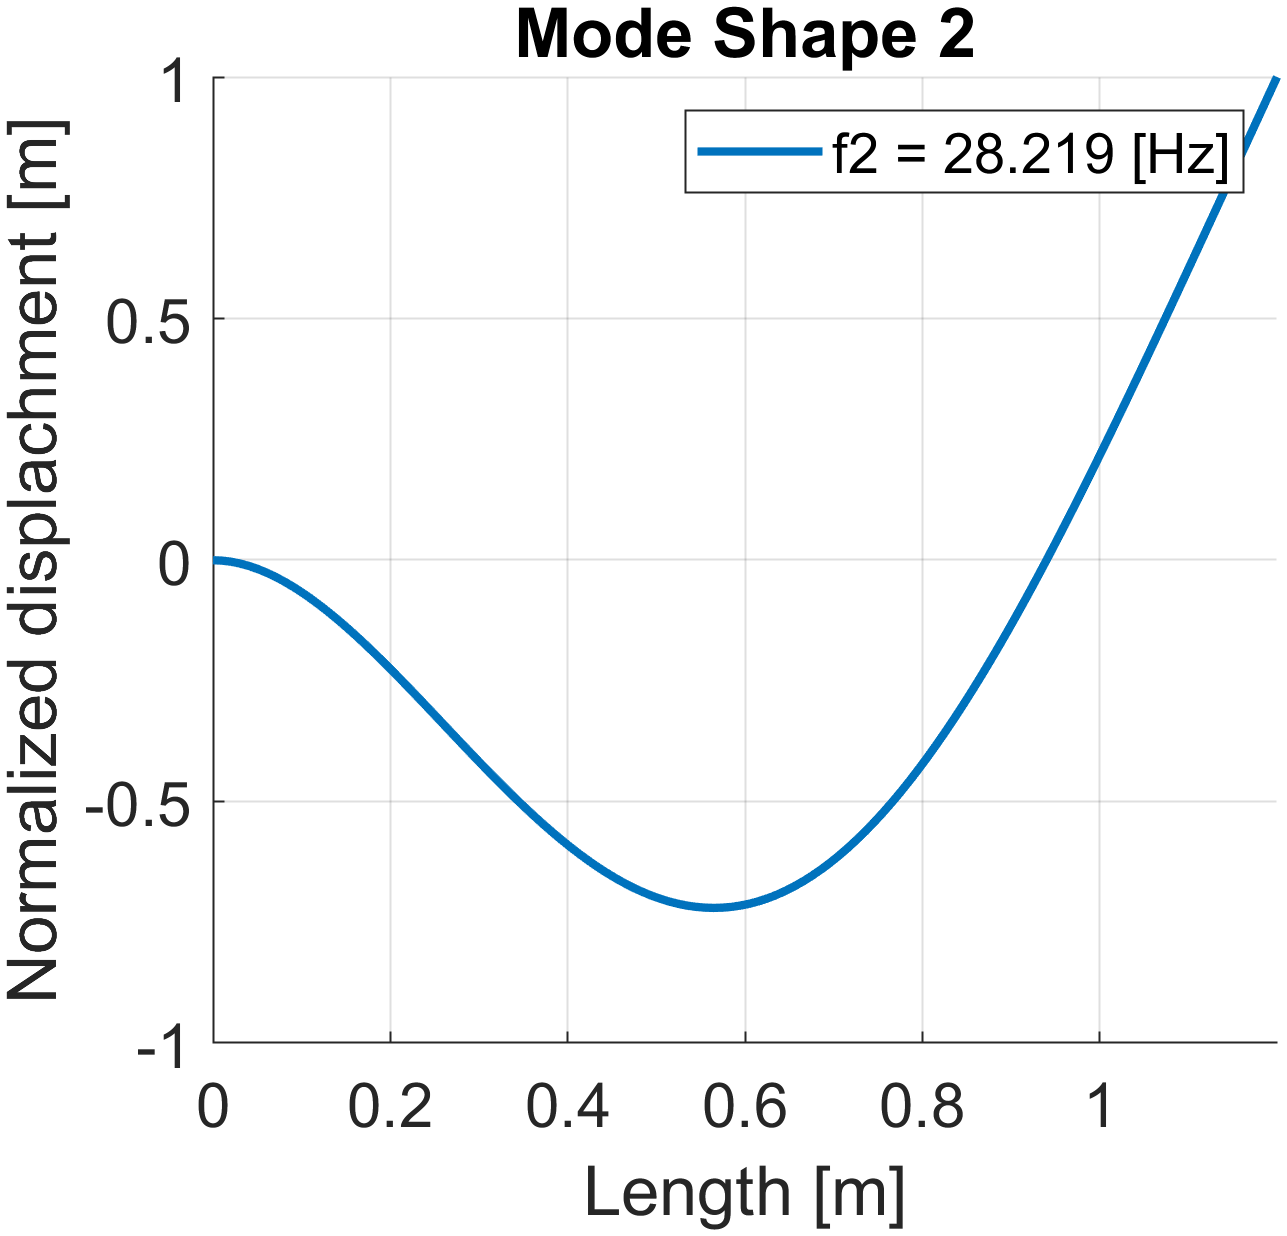
\includegraphics[width=0.9\textwidth]{img/MATLAB/Part_A/Mode_shapes/mode_shape_02.png}
    \end{minipage}
    \begin{minipage}[b]{0.45\textwidth}
        \centering
        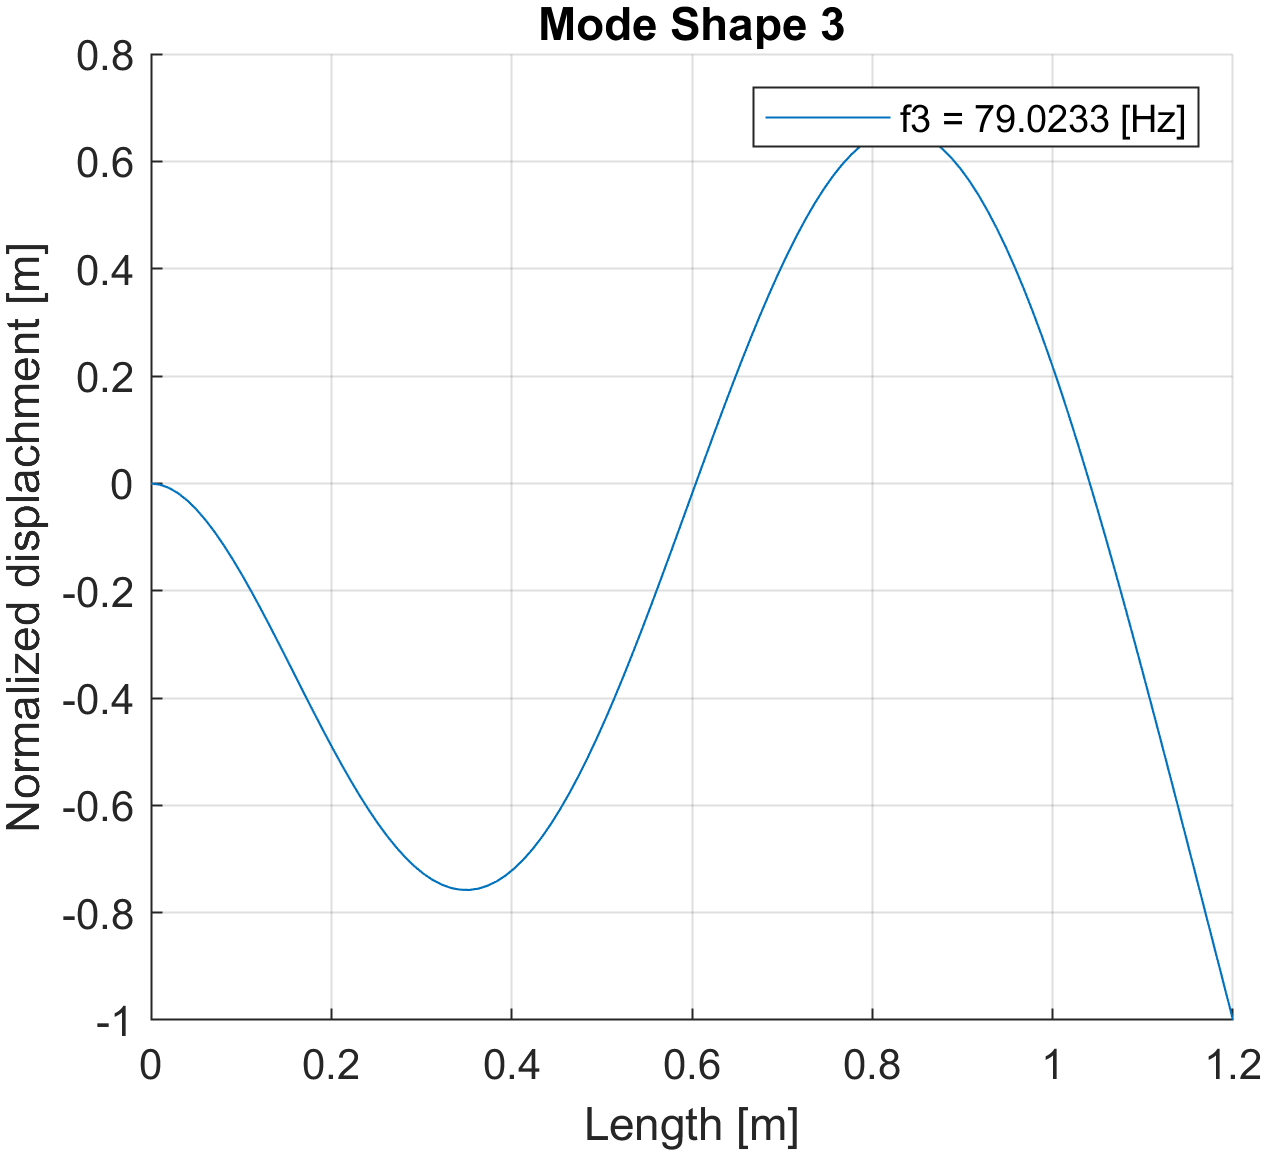
\includegraphics[width=0.9\textwidth]{img/MATLAB/Part_A/Mode_shapes/mode_shape_03.png}
    \end{minipage}
    \hfill
    \begin{minipage}[b]{0.45\textwidth}
        \centering
        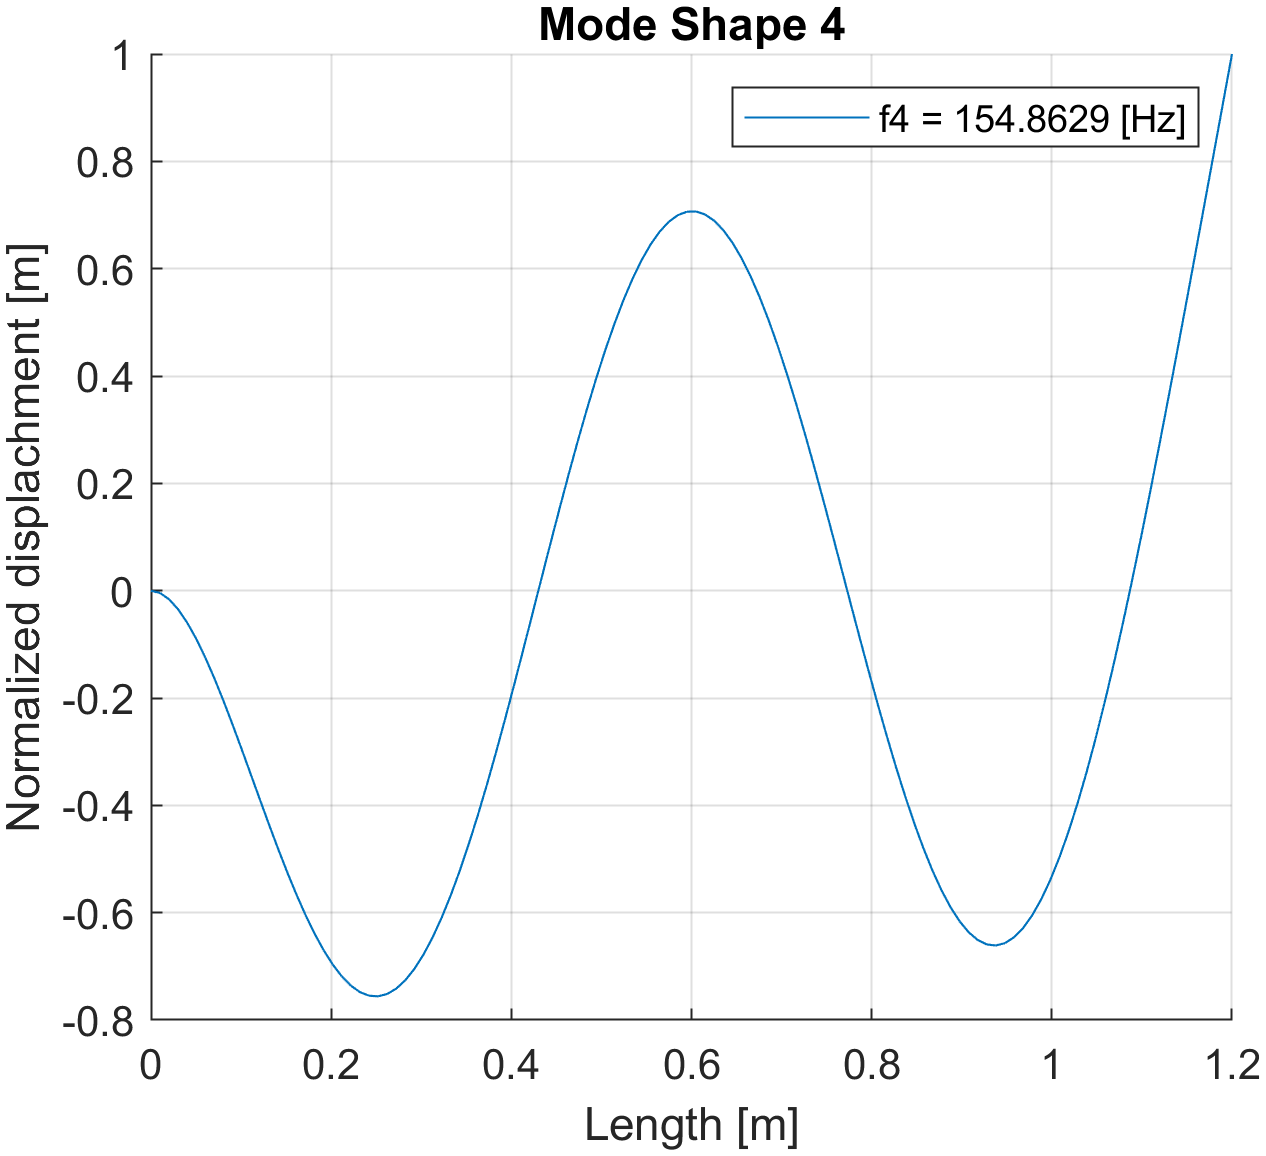
\includegraphics[width=0.9\textwidth]{img/MATLAB/Part_A/Mode_shapes/mode_shape_04.png}
    \end{minipage}
    \caption{Computed mode shapes starting from the ideal model of the cantilever beam.}
    \label{fig:ideal_mode_shapes}
\end{figure}
